% =====================================================================
% Draft section for 作業7 (paper full revision) — Results §3.6
% "System realization" — drafted to sub-subsection level with content.
% LaTeX is written to compile in BOTH the arXiv (article) and the
% TACCESS (acmart) manuscripts. Cross-refs use existing labels:
%   fig:overview, fig:arch, fig:control, fig:rate, fig:pro
% Citations use existing keys: arkit, nus, rp2040, repo.
% Degrees are written as ^{\circ} (math) and multiply as \times so no
% extra package is required.
% =====================================================================

\subsection{System realization}
\label{sec:realization}

The clinically validated control law of Section~\ref{sec:clinical} is realized
end to end by \emph{one} smartphone controller and \emph{two} interchangeable
device families (Pro for acoustic pianos, Switch for digital instruments), joined
by a deliberately simple wireless protocol and, on the Pro device, a short wired
link that separates two timing domains. This subsection describes each stage and
where the quantitative parameters (offset upper limit $3$--$10^{\circ}$,
multiplier $10$--$50$, full action within $+2$--$10^{\circ}$, and the response
speed that those two presets produce) physically live in the stack.

\subsubsection{Realized pipeline: one controller, two devices, a wired bridge}
\label{sec:pipeline}
Figure~\ref{fig:arch} summarizes the realized data path. The iOS app extracts a
head-tilt angle, applies the control law, and transmits compact messages over
Bluetooth Low Energy (BLE). On the \emph{Switch} device a single
microcontroller turns those messages directly into an electronic sustain
on/off; on the \emph{Pro} device a BLE board relays a one-byte command over a
wired UART to a second microcontroller that drives a motorized actuator against
the physical pedal. The same controller, BLE protocol, and control law serve
both devices, so an implementer learns one interaction model
(Figure~\ref{fig:overview}).

\subsubsection{iOS controller: AR face tracking and head-tilt extraction}
\label{sec:ios-ar}
The controller uses ARKit face tracking on a TrueDepth (Face~ID-class) device to
estimate head pose at roughly $60$\,fps~\cite{arkit}. A session delegate updates
a single shared head-tilt variable on every frame; the downward pitch component
is the control signal. Because face tracking is hardware-bound, the controller
runs on a physical iPhone/iPad rather than a simulator, and the screen is kept
awake during play so the foot-free session is uninterrupted.

\subsubsection{The quantitative control law in software}
\label{sec:law-sw}
The controller implements the quantitative mapping of
Section~\ref{sec:control-law} in software: each transmitted value is
$\mathrm{clamp}(0,99,(\theta-\theta_{\mathrm{off}})\times m)$ with the user's
offset $\theta_{\mathrm{off}}$ (validated $3$--$10^{\circ}$) and multiplier $m$
(validated $10$--$50$), so a further $2$--$10^{\circ}$ of tilt reaches full pedal
action (Figure~\ref{fig:control}). Engagement uses
hysteresis: an \emph{engage} event is emitted when $\theta\ge\theta_{\mathrm{off}}$
while the pedal is released, and a \emph{release} event when $\theta$ falls below
$\theta_{\mathrm{off}}$ by a small dead-band while the pedal is engaged. Because
the events are edge-triggered with a state guard, one head dip produces exactly
one engage and one release, eliminating chatter near the threshold. The
\emph{response speed} (how fast the command tracks the head beyond the offset) is
not a separate control but a secondary, temporal effect of the user's \emph{offset}
and \emph{multiplier} presets---which is what lets users with a restricted range of
motion (small offset, large multiplier) obtain a fast response.

\subsubsection{Decoupling AR sampling from BLE transmission}
\label{sec:decoupling}
The face tracker produces samples far faster than a BLE link should be driven, so
the controller \emph{decouples the two rates} (Figure~\ref{fig:rate}). The
continuous value is not sent per frame; a fixed-period timer ($\approx$100\,ms,
i.e.\ $10$\,Hz) reads the latest shared head-tilt variable and transmits it, while
the engage/release events are emitted on crossing with a short ($\approx$10\,ms)
minimum spacing. Historically the transmit period was tuned upward (from a few
milliseconds to $\approx$100\,ms) to remove a congestion/ordering fault on the
link. This producer/consumer decoupling between a fast AI sampler and a
slower wireless transport is the system's central real-time-engineering
contribution and is reused on the device side (Section~\ref{sec:coordination}).

\begin{figure}[tbp]
\centering
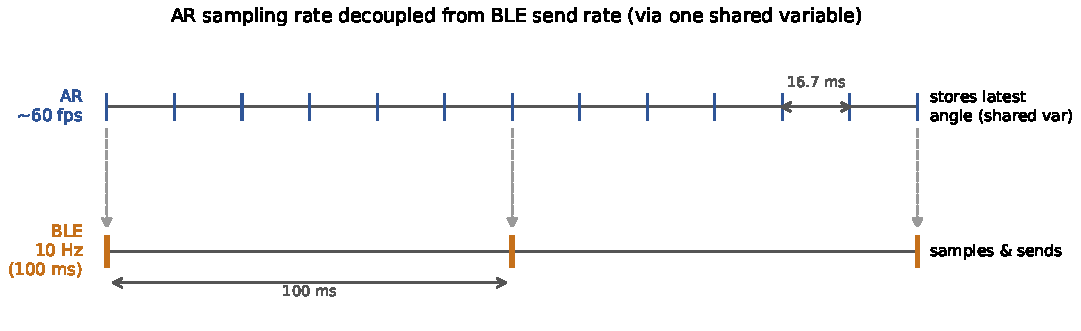
\includegraphics[width=\linewidth]{figures/fig_rate_decoupling.pdf}
\Description{Timeline comparing a dense series of AR frames at about 60 frames per
second with a sparse series of BLE transmissions at 10 hertz; the tracker updates a
shared variable that the slower timer samples and transmits.}
\caption{The fast AR sampling rate ($\sim$60\,fps) is decoupled from the slower BLE
send rate ($\sim$10\,Hz): the tracker only updates a shared variable, which a timer
samples and transmits.}
\label{fig:rate}
\end{figure}

\subsubsection{BLE link and the wire protocol}
\label{sec:ble}
The controller is a BLE central that scans, \emph{name-filters} the known device
names (\texttt{bFaaaPSwitch\_1}..\texttt{\_4}) so it never attaches to unrelated
peripherals, connects to the user-selected channel, and writes over the Nordic
UART Service (NUS)~\cite{nus} using write-without-response for low latency. The
protocol is intentionally tiny: a continuous value (\texttt{i00}..\texttt{i99}),
engage/release events, channel-rename commands, and an on-type/off-type toggle.
The play screen turns from white to red once the head passes the threshold,
giving a visual confirmation (for a helper or for setup) that matches the
device-side indicator (Section~\ref{sec:switch}).

\subsubsection{Pro device: BLE board $\rightarrow$ microcontroller $\rightarrow$ drivetrain $\rightarrow$ pedal}
\label{sec:pro-chain}
The Pro device uses two microcontrollers. An nRF52-class BLE board receives the
NUS messages and forwards a one-byte command over a wired UART to an RP2040 main
board~\cite{rp2040}. The RP2040 maps the byte to a target position between
calibrated travel limits, with a small deadband so sub-threshold jitter does not
move the motor, and drives a motor through a timing belt and a lead screw that
advances a push-rod against the sustain pedal (Figure~\ref{fig:pro}). The
result is continuous, proportional pedal depth that follows the head angle.

\begin{figure}[tbp]
\centering
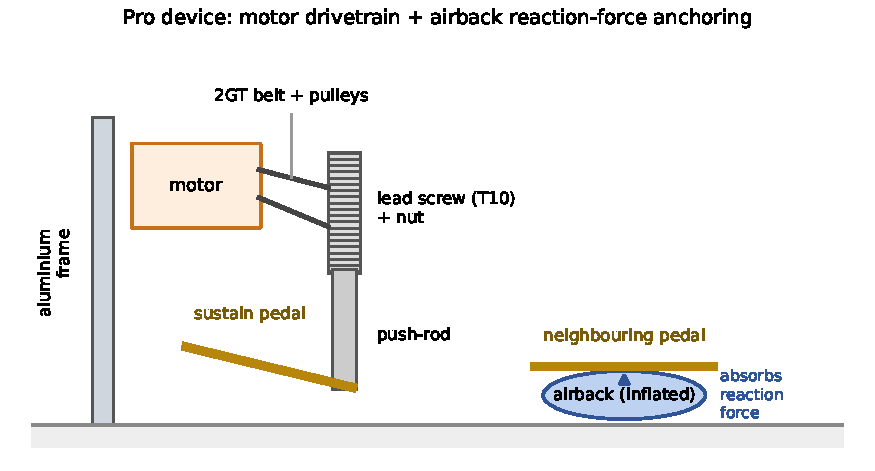
\includegraphics[width=0.92\linewidth]{figures/fig_pro_mechanism.pdf}
\Description{Side-view schematic of the Pro device. A motor on an aluminium frame
drives a timing belt and a lead screw, which lowers a push-rod onto the sustain
pedal. An inflated airback under a neighbouring pedal absorbs the upward reaction
force and anchors the unit.}
\caption{Pro device. A motor drives a timing belt and lead screw that advances a
push-rod onto the sustain pedal; an inflatable airback beneath a neighbouring pedal
absorbs the reaction force and anchors the unit on an unmodified piano.}
\label{fig:pro}
\end{figure}

\subsubsection{Reaction-force anchoring (airback) and sensorless self-calibration}
\label{sec:airback}
Two device-side mechanisms make the Pro practical on an \emph{unmodified}
acoustic piano. First, an \emph{airback} (a term we coined for an inflatable,
air-braced anchor---\emph{not} a safety ``airbag''): at power-up a pump (driven through a
power MOSFET) inflates an air bag placed under an adjacent pedal until a pressure
threshold is reached, absorbing the actuator's reaction force so the lightweight
device stays put without being bolted to the instrument (a non-destructive
anchoring). Second, \emph{sensorless self-calibration}: the actuator advances
until the motor's electrical \emph{power} --- proportional to the reaction force,
and chosen over current because power is robust to supply-voltage variation
(current alone changes with the input voltage) --- reaches a limit, which
automatically fixes the lower travel end; the upper end is set live by a slider on
a small hand controller. These two ends correspond directly to the offset (zero)
and the full-press depth of the control law.

\subsubsection{Switch device: electronic sustain switching for digital instruments}
\label{sec:switch}
For digital pianos and keyboards the Switch device needs no motor, drivetrain, or
airback. The BLE board drives a GPIO pin into a relay/optocoupler that opens or
closes the instrument's sustain jack, so the same engage/release events that move
a motor on the Pro instead toggle an electronic sustain. An on-board RGB LED
mirrors the controller's white$\rightarrow$red feedback (idle / armed / engaged),
and the on-type/off-type toggle accommodates the jack polarity of different
instruments.

\subsubsection{End-to-end coordination and timing budget}
\label{sec:coordination}
On the Pro device the wired UART bridges an \emph{asynchronous} wireless domain
(the BLE board, whose radio stack is event-driven) and a \emph{synchronous}
motion domain (the RP2040, which runs a deterministic blocking loop) --- the same
decoupling philosophy as the iOS AR/BLE split (Section~\ref{sec:decoupling}). The
budget holds in the field: in a real grand-piano session the controller emitted
on the order of two thousand continuous values and an equal count of engage and
release events (one per head dip) with no transmission errors and no
desynchronization, confirming that the $10$\,Hz value stream plus throttled
events stay within what the link and the actuator can absorb.
